\section{Kradzież tożsamości}
\begin{frame}{Kradzież tożsamości}
\begin{columns}[c]
    \column{.55\textwidth}
    \begin{block}{Co może się wydarzyć?}
    \begin{itemize}
    \item Pożyczki i konta bankowe na nasze dane
    \item Oszustwa zdrowotne i podatkowe
    \item Długoterminowe problemy finansowe
    \end{itemize}
    \end{block}
    \column{.45\textwidth}
    \centering
    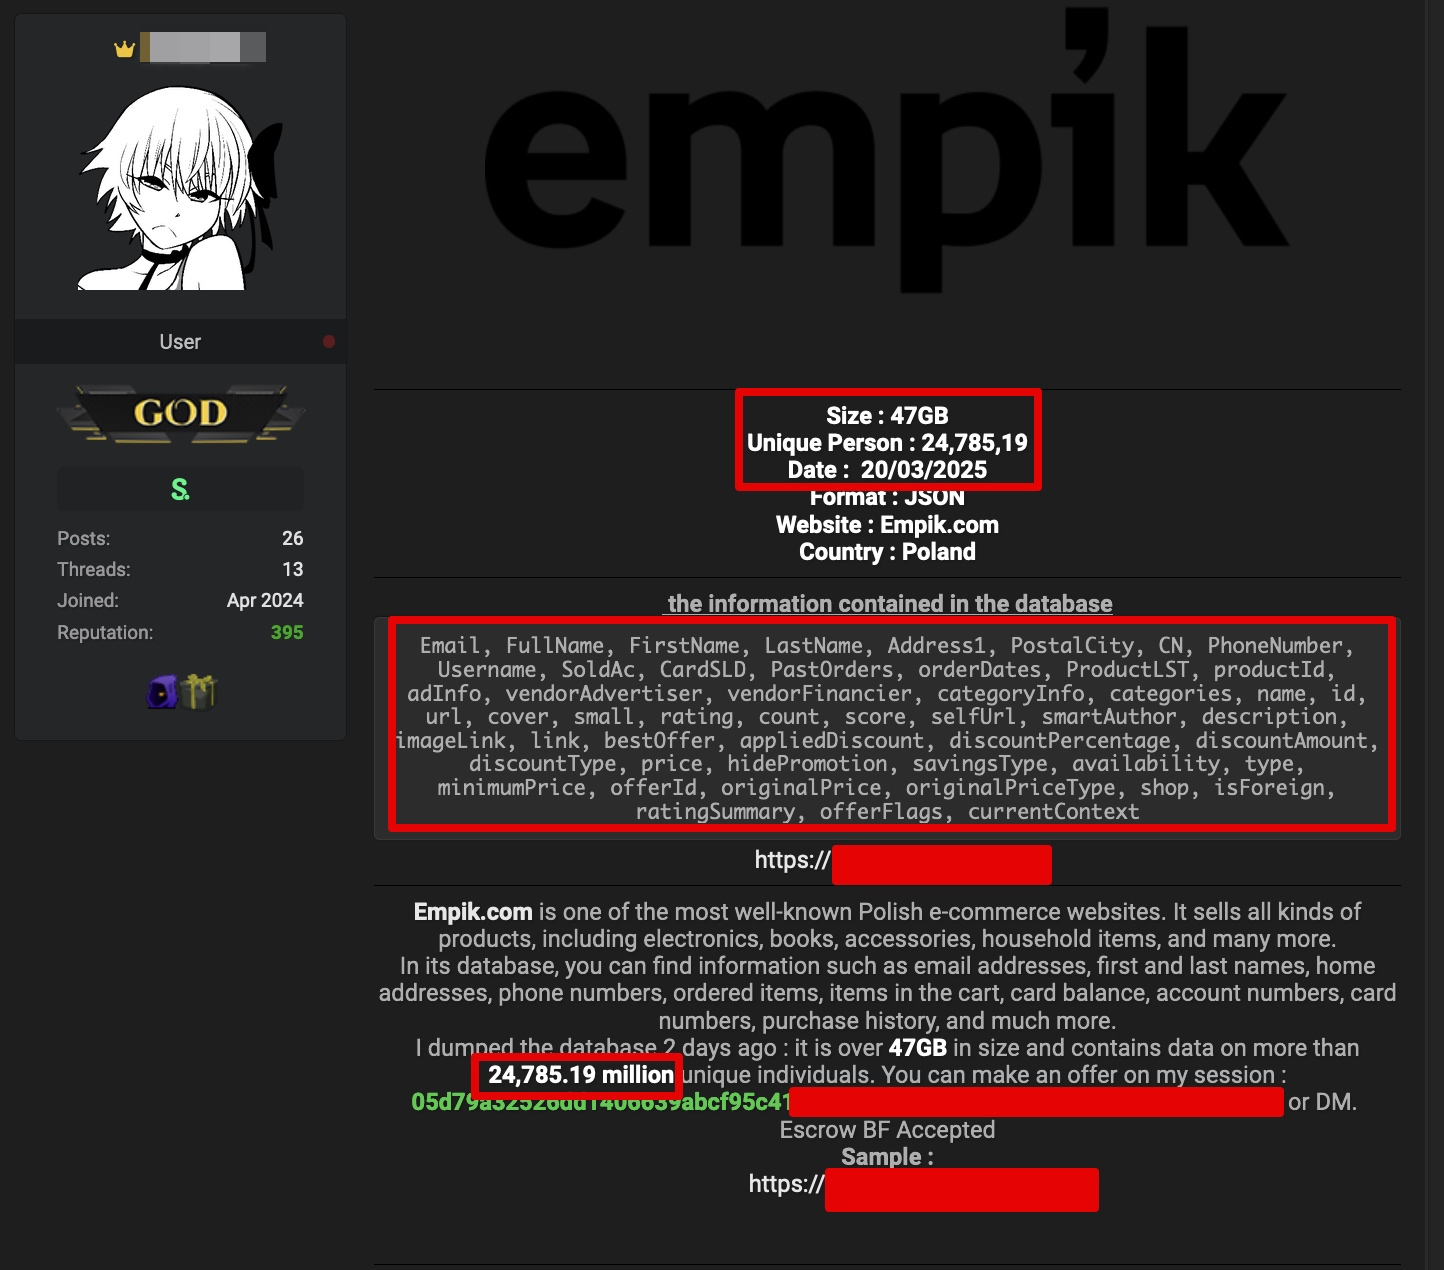
\includegraphics[width=1\textwidth]{images/empik-wyciek.jpg}
\end{columns}
\end{frame}

\begin{frame}{Pomyłka i hejt: Propine Case}
\begin{columns}[c]
    \column{.6\textwidth}
    \begin{itemize}
      \item Fałszywa identyfikacja CEO
      \item Publikacja zdjęć, adresu, telefonu
      \item Fala gróźb i rasistowskich ataków
    \end{itemize}
    \begin{alertblock}{Wniosek}
    Jedna pomyłka w social media = fala nienawiści
    \end{alertblock}
    \column{.4\textwidth}
    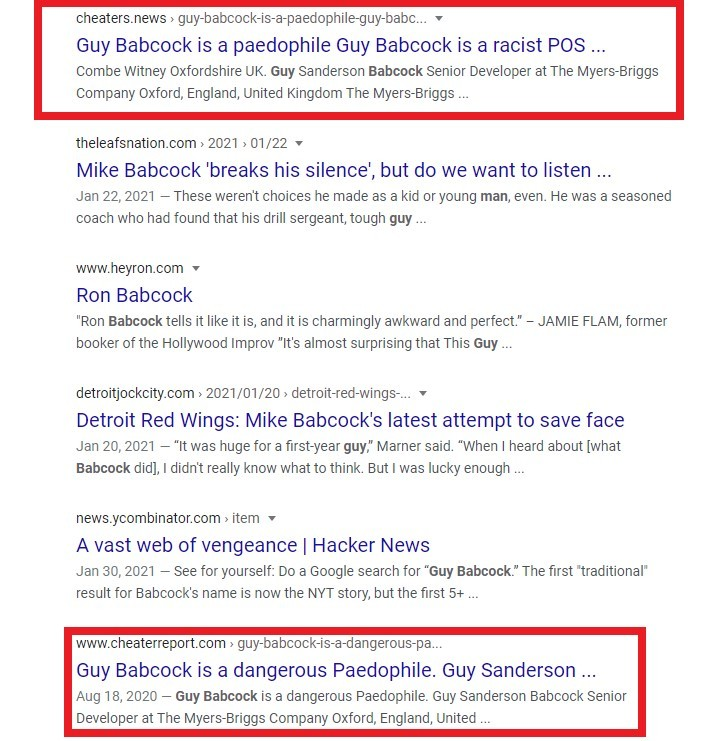
\includegraphics[width=0.75\textwidth]{images/pedophile.jpg}
\end{columns}
\end{frame}

\section{Naruszenie prywatności}
\begin{frame}{Naruszenie prywatności}
\begin{columns}[c]
    \column{.55\textwidth}
    \begin{itemize}
      \item Utrata kontroli nad danymi
      \item Publiczne rozpowszechnianie danych
      \item Ryzyko monitorowania i śledzenia
    \end{itemize}
    \column{.45\textwidth}
    \centering
    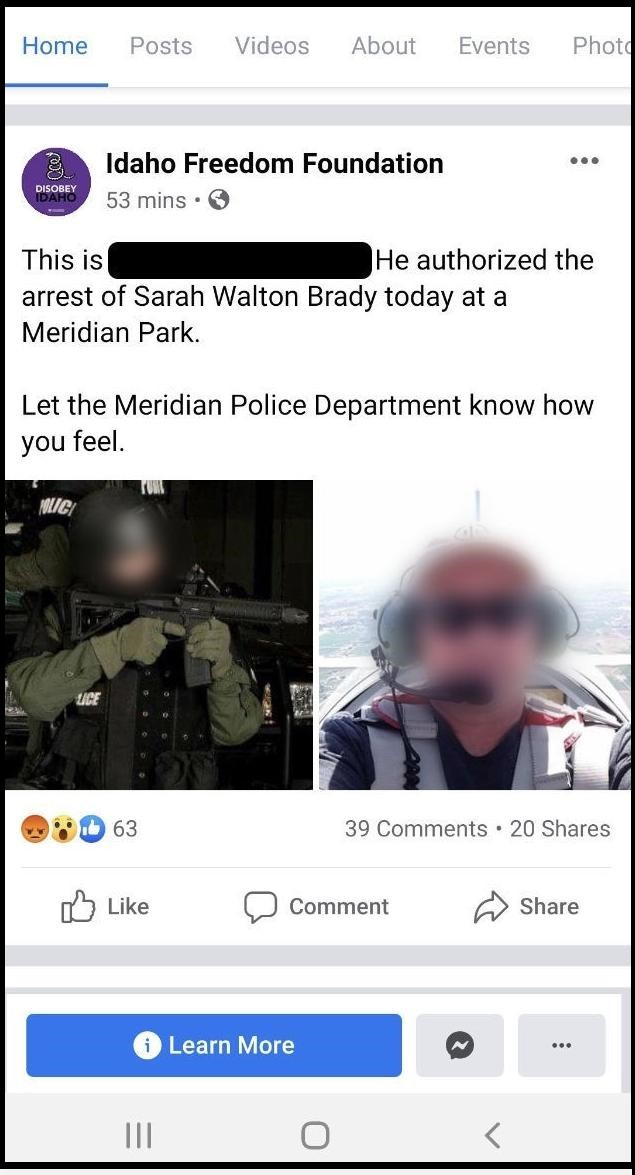
\includegraphics[width=0.5\textwidth]{images/officer.jpg}
\end{columns}
\end{frame}

\begin{frame}{Case: Empik}
\begin{columns}[c]
    \column{.5\textwidth}
    \begin{exampleblock}{Empik: Reakcja wzorcowa}
    \begin{itemize}
      \item Szybka analiza
      \item Komunikacja z klientami
      \item Współpraca z zespołem CERT \cite{empik}
    \end{itemize}
    \end{exampleblock}
    \column{.5\textwidth}
    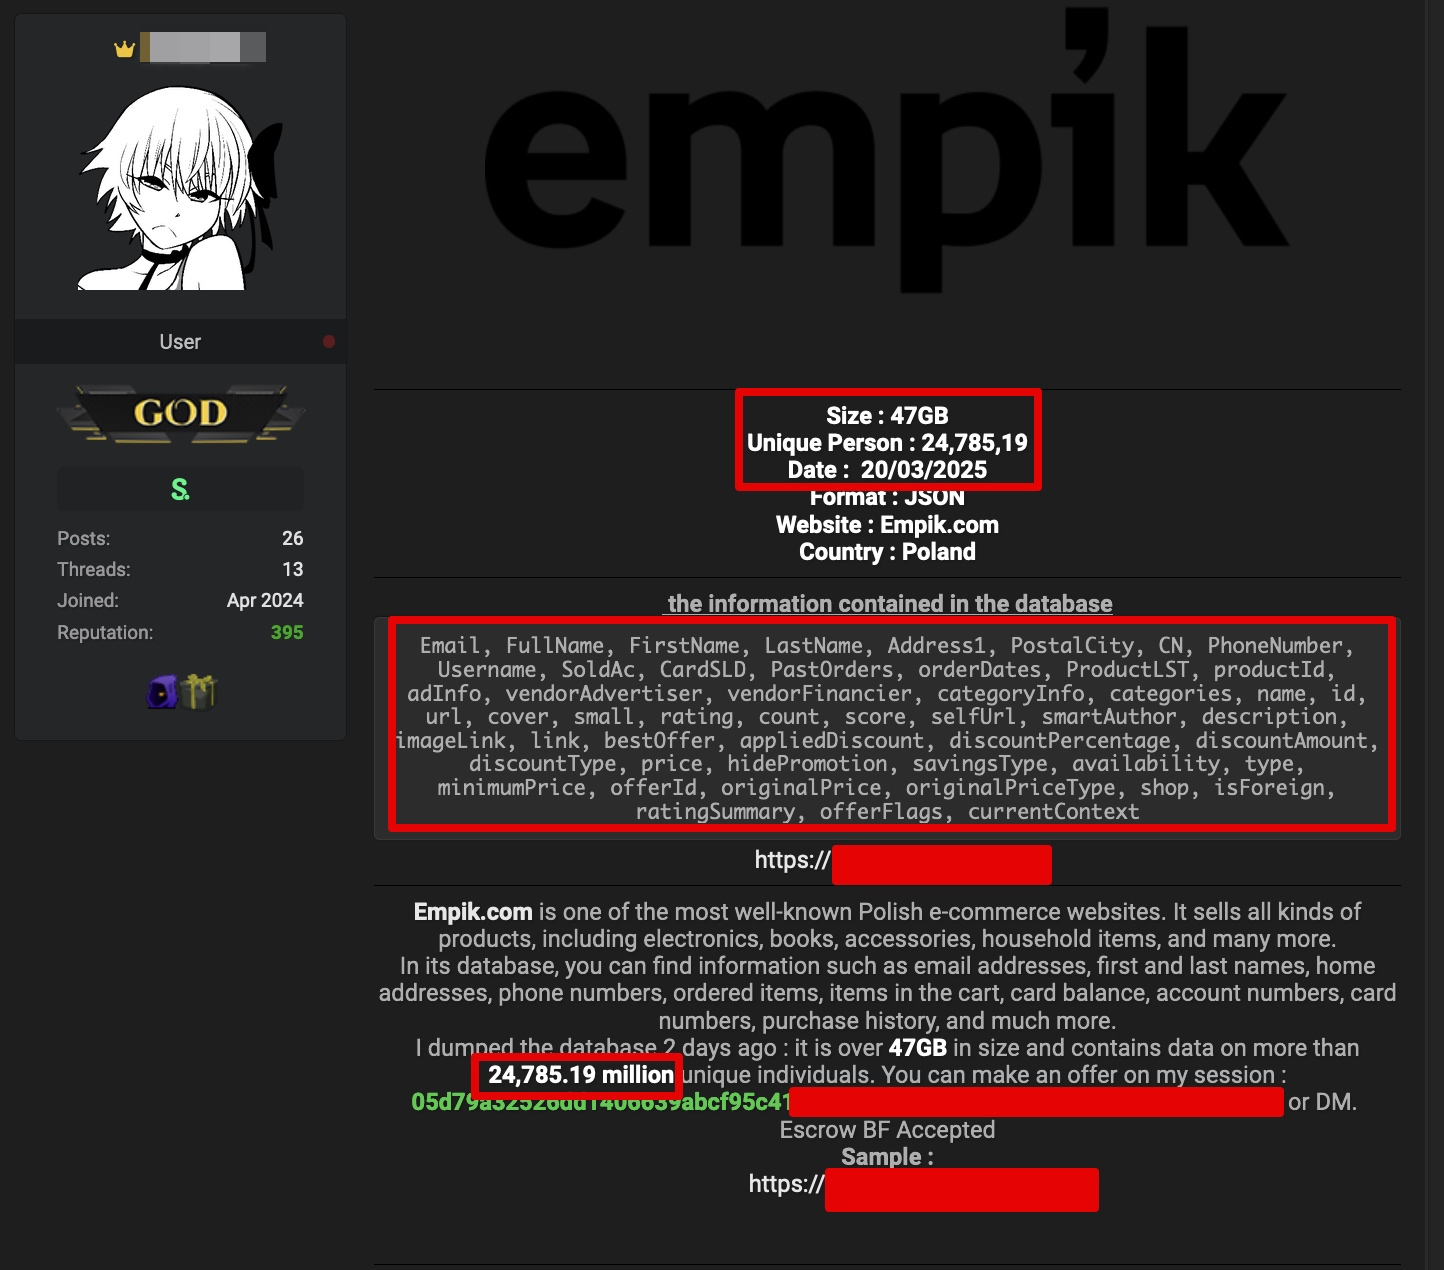
\includegraphics[width=1\textwidth]{images/empik-wyciek.jpg}
\end{columns}
\end{frame}

\section{Cyberstalking}
\begin{frame}{Cyberstalking}
\begin{columns}[c]
    \column{.55\textwidth}
    \begin{itemize}
      \item Ujawnienie danych = nękanie offline
      \item Groźby, wandalizm, zastraszanie
      \item Strach, trauma, izolacja
    \end{itemize}
    \column{.45\textwidth}
    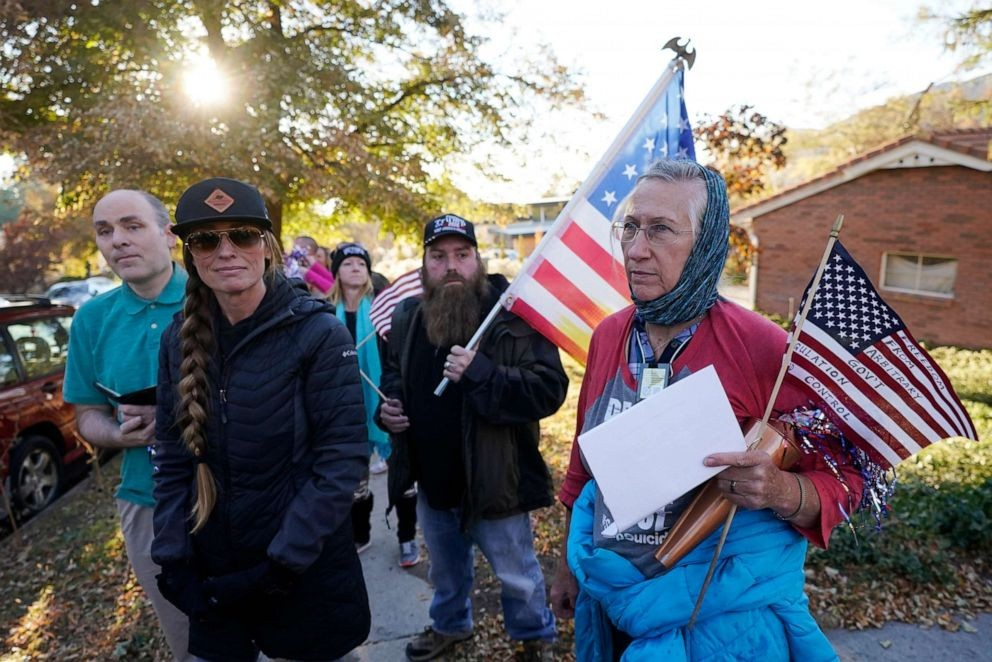
\includegraphics[width=1\textwidth]{images/lockdown.jpg}
\end{columns}
\end{frame}

\section{Oszustwa socjotechniczne}
\begin{frame}{Oszustwa socjotechniczne}
\begin{columns}[c]
    \column{.55\textwidth}
    \begin{itemize}
      \item Phishing i vishing
      \item Podszywanie się pod pracowników firm
      \item Tworzenie fałszywych tożsamości
    \end{itemize}
    \column{.45\textwidth}
    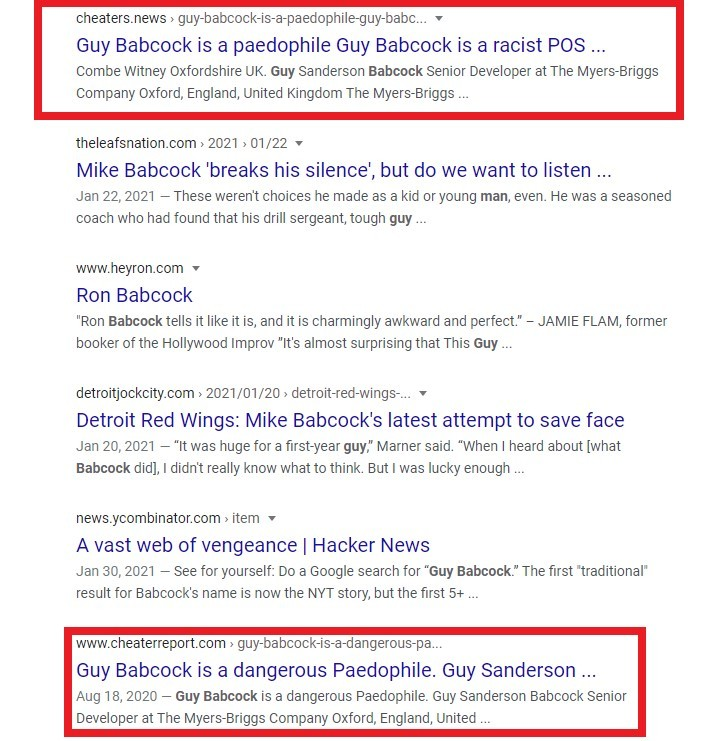
\includegraphics[width=0.75\textwidth]{images/pedophile.jpg}
\end{columns}
\end{frame}

\section{Reputacja i odpowiedzialność}
\begin{frame}{Utrata reputacji}
\begin{columns}[c]
    \column{.55\textwidth}
    \begin{itemize}
      \item Media, nagłówki, skandale
      \item Trudności zawodowe
      \item Publiczne lincze i dezinformacja
    \end{itemize}
    \column{.45\textwidth}
    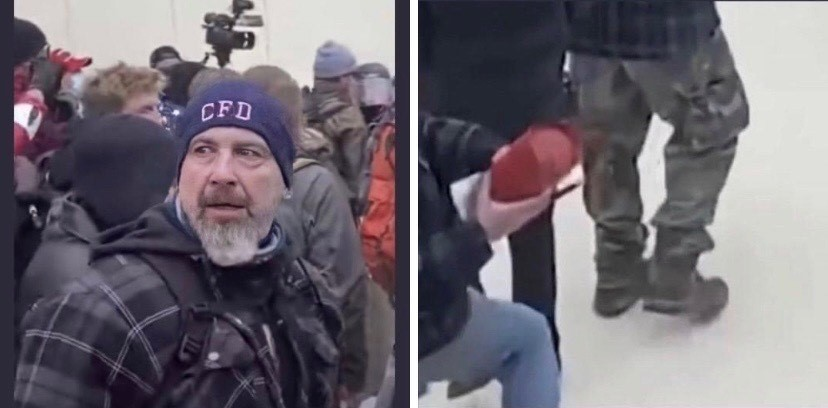
\includegraphics[width=1\textwidth]{images/david.jpg}
\end{columns}
\end{frame}

\begin{frame}{Odpowiedzialność prawna}
    \begin{block}{Ryzyko prawne}
        \begin{itemize}
        \item Pozwy cywilne
        \item Kara za naruszenia RODO
        \item Odpowiedzialność karna \cite{zagrozeniaLudzie}
        \end{itemize}
    \end{block}
\end{frame}